Authentication flow diagram
\begin{figure}[H]
    \centering
    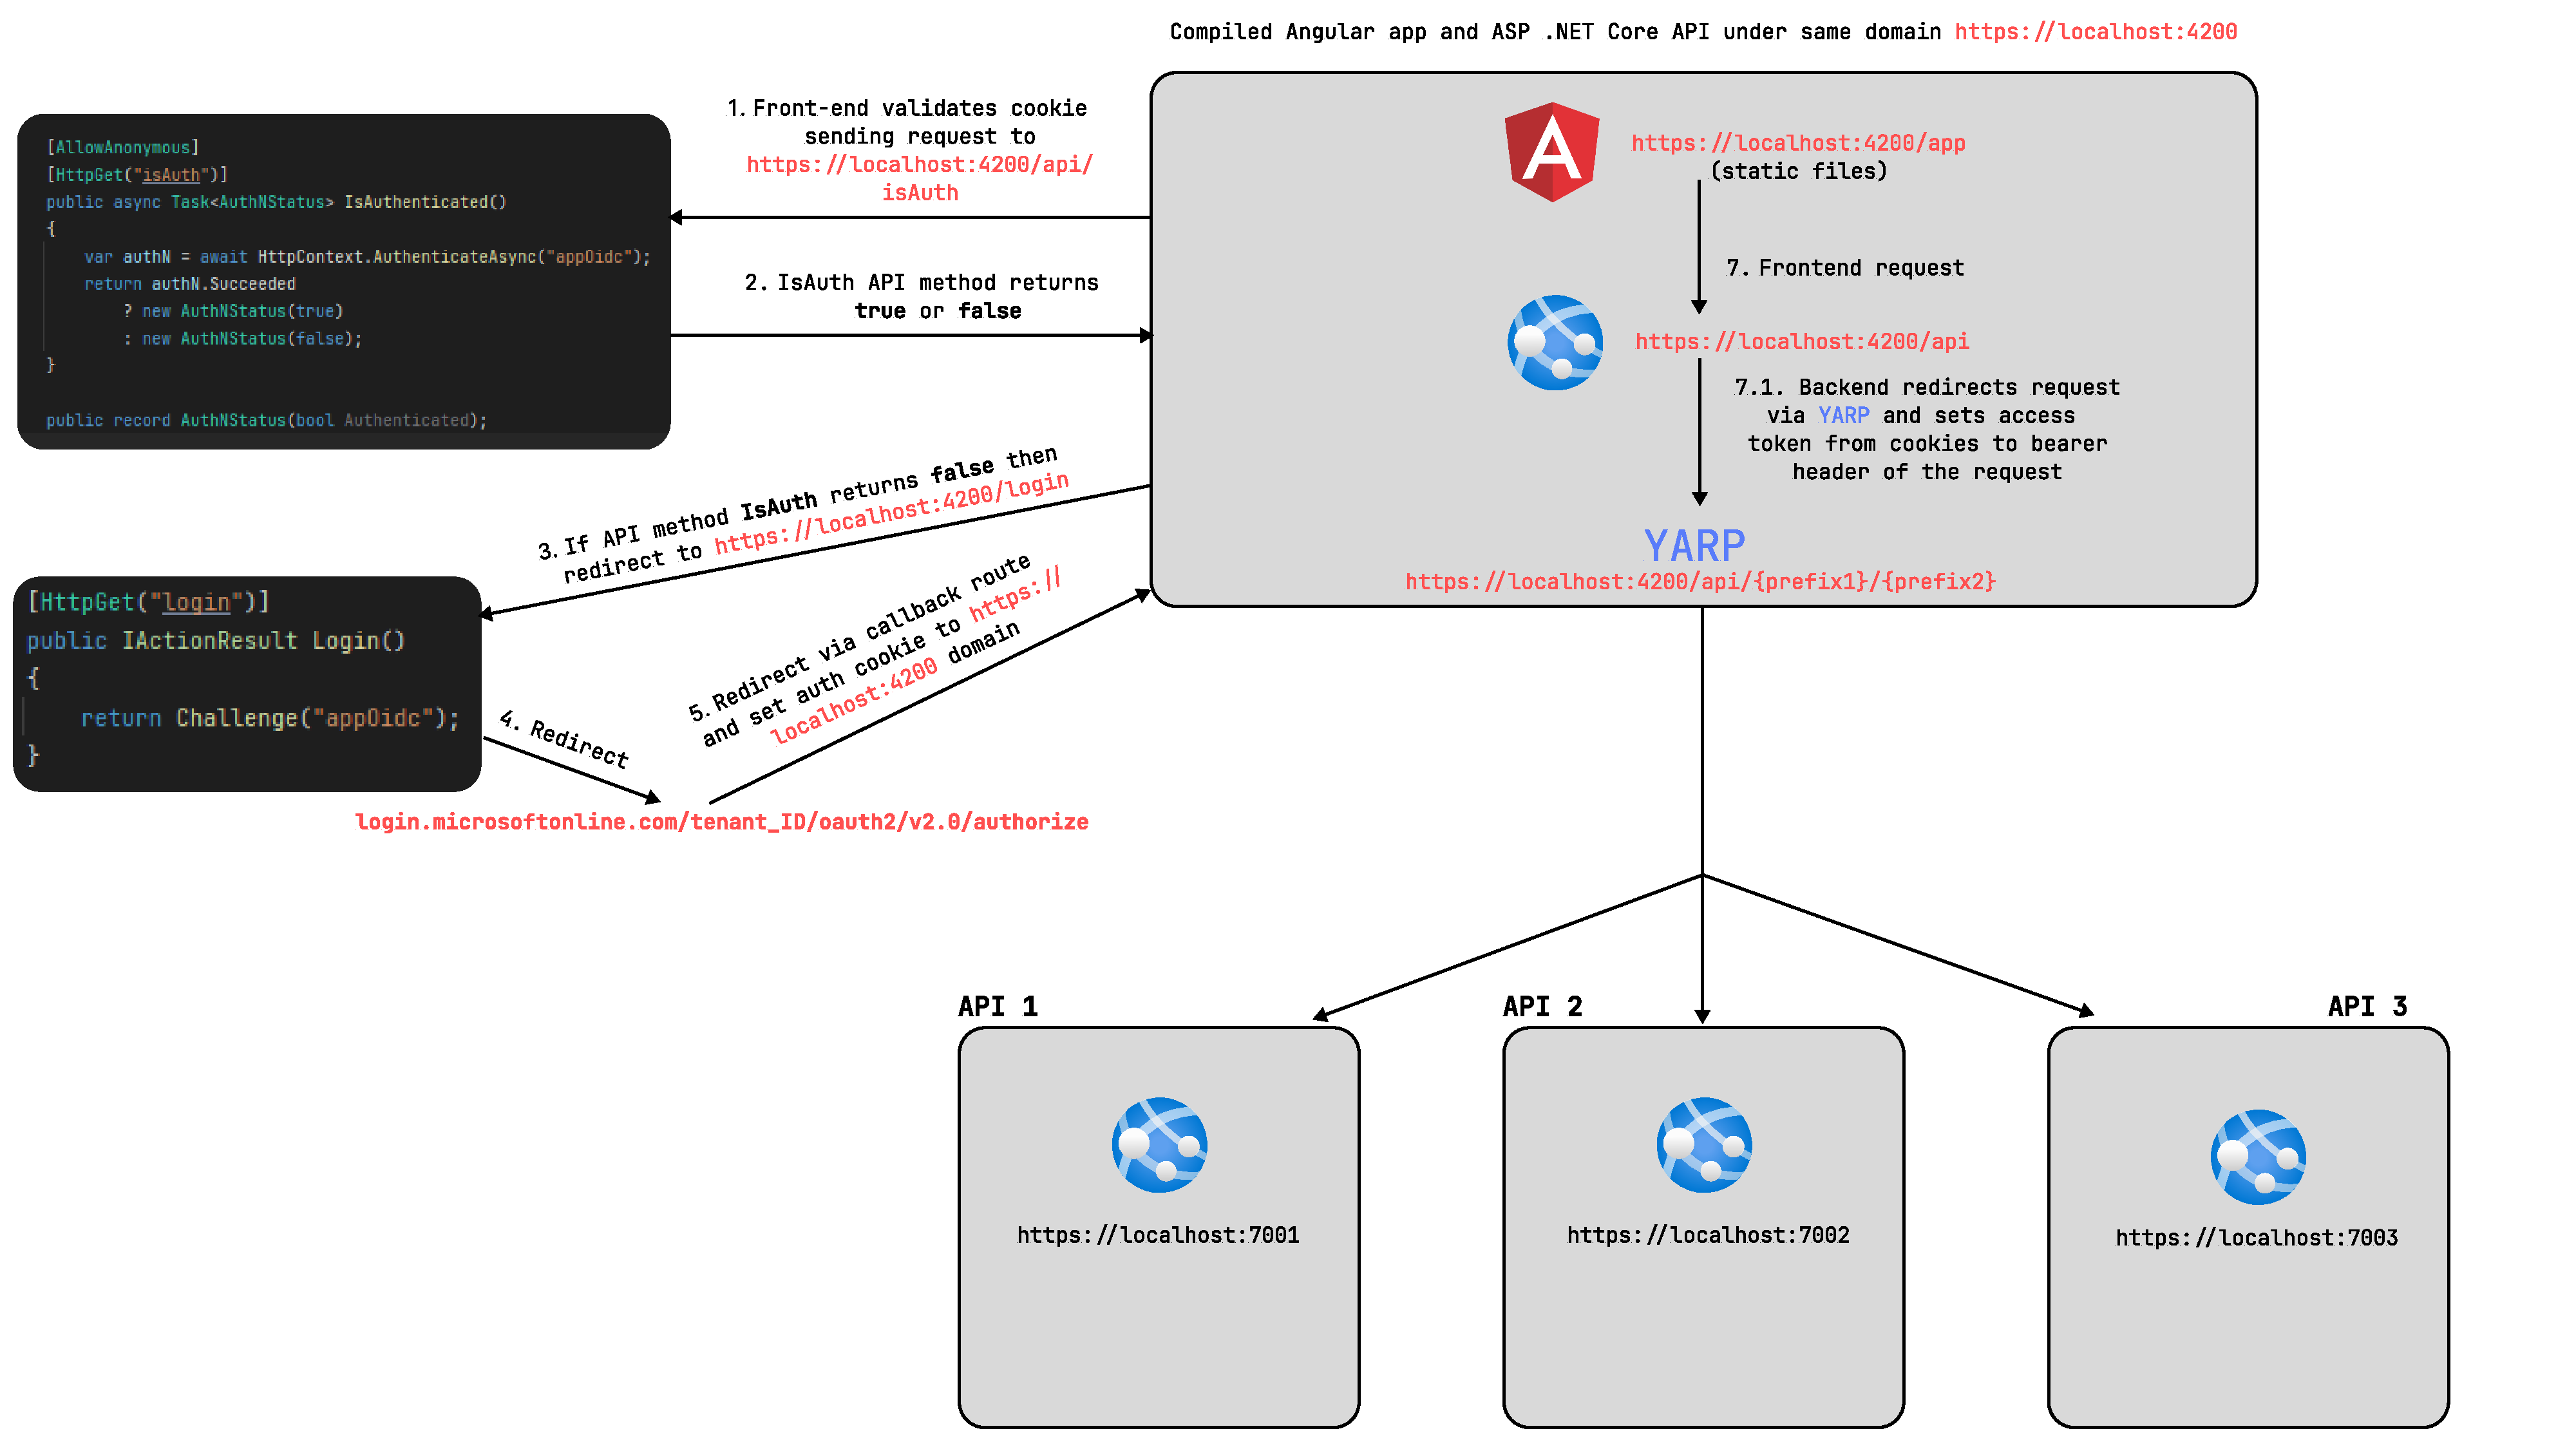
\includegraphics[width=1\textwidth]{img/Auth_flow_updated}
    ~\caption{Authentication flow diagram.}\label{fig:authentication_flow_diagram}
\end{figure}

\begin{enumerate}
    \item Frontend application sends request to \texttt{https://localhost:4200/api/isAuth} API method to validate authentication
    \item API method \texttt{https://localhost:4200/api/isAuth} returns \texttt{true} if authentication valid, otherwise \texttt{false}
    \item If authentication invalid then browser redirects to \texttt{https://localhost:4200/login}, otherwise no action taken
    \item Login redirects browser to authorize url \\
    \texttt{login.microsoftonline.com/tenant/oauth2/v2.0/authorize}
    \item If user is logged in then browser is redirected to fallback url with cookies already set for \texttt{https://localhost:4200} domain
    \item Request is sent to validate authentication \texttt{https://localhost:4200/api/isAuth}, now it returns \texttt{true}
    \item Frontend at \texttt{https://localhost:4200/app} sends request to the \\ \texttt{https://localhost:4200/api/OtherApi1/products}
    \item Cookie exists for \texttt{https://localhost:4200/app} so that \\ \texttt{https://localhost:4200/api}
    attaches it as header to request via YARP and sends request with token to the external resource \texttt{OtherApi1/products}
    \item If response code is 401 at step (8) then repeat step (1)
\end{enumerate}